%\numberwithin{equation}{part}
%\numberwithin{equation}{section}

%\graphicspath{{pictures/}}
%\DeclareGraphicsExtensions{.pdf,.png,.jpg}

%\tableofcontents
%\newpage

\newenvironment{Proof} 	% имя окружения
	{\par\noindent{\bf Доказательство.}}  % команды для \begin 
	{\hfill$\scriptstyle\blacksquare$}

\section{Теоретические основы}
\label{sec:theoretical}
\subsection{Система передачи информации. Общая схема (кодер источника - кодер канала – модулятор – канал - декодер канала – демодулятор - декодер)} %%Скляр
\subsubsection{Система передачи информации.Общая схема}
Передача информации происходит от источника к получателю (приемнику) информации. {\bf Источником} информации может быть все, что угодно: любой объект или явление живой или неживой природы. Процесс передачи информации протекает в некоторой материальной среде, разделяющей источника и получателя информации, которая называется {\it каналом} передачи информации. Информация передается через канал в форме некоторой последовательности сигналов, символов, знаков, которые называются {\it сообщением}. {\bf Получатель информации} — это объект, принимающий сообщение, в результате чего происходят определенные изменения его состояния.\\
Клодом Шенноном была предложена модель процесса передачи информации по техническим каналам связи, представленная схемой:
\begin{figure}[h]
\center{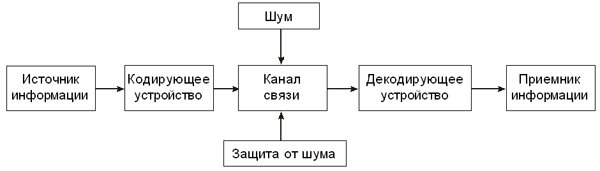
\includegraphics[scale=0.7]{1_4.jpg}}
\caption{Техническая система передачи информации}
\label{fig:image}
\end{figure} \\\indent
Под кодированием здесь понимается любое преобразование информации, идущей от источника, в форму, пригодную для ее передачи по каналу связи. {\bf Декодирование} — обратное преобразование сигнальной последовательности.\\\indent
Термином “шум” называют разного рода помехи, искажающие передаваемый сигнал, затухание, зашумление, частотная расинхронизация, искадения, связанные с многолучевым распространением и приводящие к потере информации. Такие помехи прежде всего возникают по техническим причинам: плохое качество линий связи, незащищенность друг от друга различных потоков информации, передаваемых по одним и тем же каналам.Наличие шума приводит к потере передаваемой информации. В таких случаях необходима защита от шума.  
Также в общую схему системы передачи информации входит {\it модулятор} и {\it демодулятор}.\\\indent
{\bf Модулятор} (лат. {\it modulator} — соблюдающий ритм) — устройство, изменяющее параметры несущего сигнала в соответствии с изменениями передаваемого (информационного) сигнала. Этот процесс называют модуляцией, а передаваемый сигнал модулирующим.

{\bf Демодуляция} ({\bf Детектирование сигнала}) — процесс, обратный модуляции колебаний, выделение информационного (модулирующего) сигнала из модулированного колебания высокой (несущей) частоты.

%\subsubsection{Схема кодера}
%\begin{figure}[h]
%\center{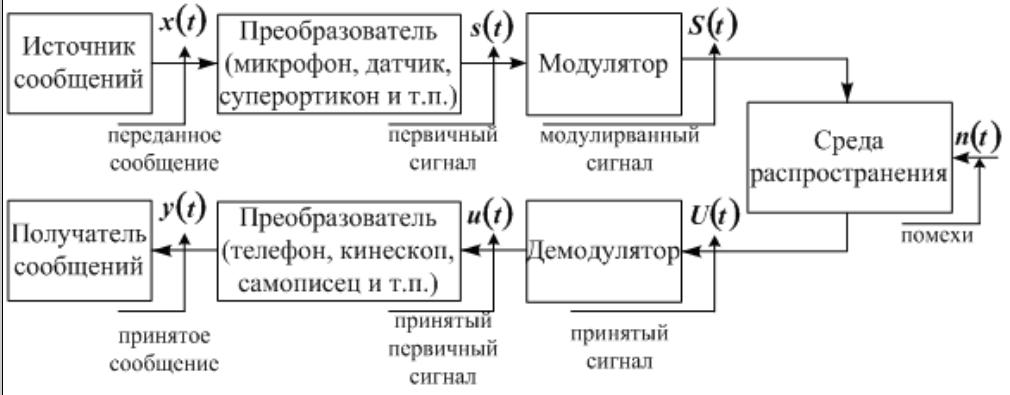
\includegraphics[scale=0.7]{1_5.jpg}}
%\caption{Техническая система передачи информации}
%\label{fig:image}
%\end{figure

%\subsubsection{Схема декодера}
%\begin{figure}[h]
%\center{\includegraphics[scale=0.7]{1_6.jpg}}
%\caption{Техническая система передачи информации}
%\label{fig:image}
%\end{figure
\newpage

\subsection{Преобразование Фурье, виды преобразования Фурье}
Электрические сигналы связи - это меняющиеся со временем сигналы напряжения или тока, обычно описываемые во временной области. Кроме того, подобные сигналы также удобно описывать в частотной области, где описание сигнала называется его {\it спектром}. Спектральные понятия важны при анализе и проектировании систем связи; они могут описывать сигнал через его среднюю мощность или энергетическое содержание на различных частотах и показывают, какую часть (полосы) электромагнитного спектра занимает сигнал. Если говориться, что конкретный спектр описывает сигнал, подрузамевается, что один из способов описания сигнала - это задать его амплитуду и фазу как функции частоты.\\\indent {\it Преобразование Фурье} (Fourier transform) является инструментом спектрального анализа сигналов. \\\indent Сигнал может предсталяться как переодической или непереодической функцией, так и неким прямоугольным изображением $B(x,y)$, где $ 0 \leq x\leq X$, $0 \leq y\leq Y$, $B(x',y')$ - яркость пиксела с координатами $(x',y')$ %%(нужно ли писать виды сигналов?)

 %%Скляр + Сергиенко
\subsubsection{Преобразование Фурье. Основные свойства} %Романюк
Введем основные определения и свойства преобразования Фурье.\\
Пусть $x(t)$ - функция периодического сигнала с конечной энергией:

$$
\int\limits_{-\infty}^{\infty}|x(t)|^2dt < \infty 
$$
\indent Известно, что для существования преобразования Фурье достаточно выполнение следующих условий Дирихле:


%\renewcommand{\listi} {
	% вертикальные промежутки:
	%\topsep=0pt % вокруг списка
	%\parsep=0pt % между абзацами
	%\itemsep=0pt % между пунктами
	% горизонтальные промежутки:
	%\itemindent=0pt % абзацный выступ
	%\labelsep=1ex % расстояние до метки
	%\leftmargin=\parindent % отступ слева
	%\rightmargin=0pt % отступ справа 
	%}
\begin{enumerate}%[16]-Романюк
	\renewcommand{\theenumi}{(\asbuk{enumi})}
	\renewcommand{\labelenumi}{\asbuk{enumi})}
	\item $x(t)$ ограничена при $t\in(-\infty,\infty);$
	\item $x(t)$ абсолютно интегрируема на $(-\infty,\infty);$
	\item $x(t)$ имеет конечное число максимумов и минимумов, а также конечное число разрывов на каждом конечном интервале.
\end{enumerate}
\indent Имеет место {\it теорема Планшереля}: если $x(t)$ - функция с интегрируемым квадратом на всей оси, то существует  функция $x(t)$ также с интегрируемым квадратом на всей оси и связанная с $X(f)$ соотношением
$$
X(f) = l.i.m._{T\to\infty} \int\limits_{-T}^{T}x(t)e^{-j2 \pi ft}dt, 
$$
где l.i.m понимается как предел в среднем(limit in the mean):
$$
\lim_{T\to\infty}  \int\limits_{-\infty}^{\infty}\left|X(f)- \int\limits_{-T}^{T}x(t)e^{-j2 \pi ft}\right|^2df = 0. 
$$
\indent Аналогично, если $X(f)$ - функция с интегрируемым квадратом на всей оси, то существует функция $x(t)$ также с интегрируемым квадратом на всей оси и связанная с $X(f)$ соотношением
$$
x(t) = l.i.m._{W\to\infty} \int\limits_{-W}^{W}X(f)e^{j2 \pi ft}df, 
$$
В этом случае имеет место равенство Парсеваля:
$$
\int\limits_{-\infty}^{\infty}|x(t)|^2dt = \int\limits_{-\infty}^{\infty}|X(f)|^2df  
$$
Кроме того, если $x(t)$ абсолютно интегрируема, то
$$
X(f) = \int\limits_{-\infty}^{\infty}x(t)e^{-j2 \pi ft}dt, 
$$
Если и функция $X(f)$ абсолютно интегрируема, то
$$
x(t) = \int\limits_{-\infty}^{\infty}X(f)e^{j2 \pi ft}df, 
$$
Соотношения (6) и (7) определяют пару преобразований Фурье соотвественно {\it прямое} и {\it обратное}.
\\\indent Для частоты $\omega = 2 \pi f$ пара преобразований Фурье имеет следующий вид:
\begin{gather}
  X(\omega) = \int\limits_{-\infty}^{\infty}x(t)e^{-j\omega t}dt, \\ 
  x(t) = \frac{1}{2\pi} \int\limits_{-\infty}^{\infty}X(\omega)e^{j\omega t}d\omega
\end{gather}
\indent Интеграл (8) называется {\it спектральной плотностью}, а интеграл (9) - интегралом Фурье.\\
\begin{center}
	{\bf Свойства спектральной плотности}
\end{center}
\begin{enumerate}
	\renewcommand{\labelenumi}{\arabic{enumi})}
	\item В общем случае $X(\omega)$ - {\it комплексная функция} частосты
	$$
		X(\omega) = Re\left[X(\omega)\right] - jIm\left[X(\omega)\right] = A(\omega)-jB(\omega) = \left|X(\omega)\right]e^{j\varphi(\omega)}
	$$
	где 
	\begin{align}
		A(\omega) = Re\left[X(\omega)\right] = \int\limits_{-\infty}^{\infty}x(t){\cos \omega t}dt \\
		B(\omega) = Im\left[X(\omega)\right] = \int\limits_{-\infty}^{\infty}x(t){\sin \omega t}dt \\
		\left|X(\omega)\right| = \sqrt{A^2(\omega) + B^2(\omega)} 
	\end{align}
	-{\it амплитудно-частотная характеристика} (АЧХ),
		$$\varphi(\omega) = -{\arctg \frac{B(\omega)}{A(\omega)}} $$
	-{\it фазочастотная характеристика} (ФЧХ) спектральной плотности сигнала.
	\item {\it Свойства симметрии} $X(\omega).$  Для действительного сиглана (физические сигналы всегда действительные функции) имеет место $$X(\omega)=X*(-\omega) $$
	\item {\it Полезные соотношения.} Для действительного сигнала $x(t)$ имеет место 
	$$
	x(t) = \frac{1}{2\pi} \int\limits_{-\infty}^{\infty}X(\omega)e^{j\omega t}d\omega = \frac{1}{2\pi} \int\limits_{-\infty}^{\infty}\left|X(\omega)\right|e^{j\left[\omega t + \varphi(\omega)\right]}d\omega = \frac{1}{\pi} \int\limits_{0}^{\infty}\left|X(\omega)\right| {\cos \left[\omega t + \varphi(\omega)\right] }d\omega.
	$$
	При $\omega = 0\  X(0) = \int\limits_{-\infty}^{\infty}x(t)dt $ - площадь сигнала.\\
	При $t=0\  x(0) = \int\limits_{-\infty}^{\infty}X(\omega)d\omega.$
\end{enumerate}

\begin{center}
	{\bf Основные спектральные теоремы}
\end{center}
\begin{enumerate}
	\renewcommand{\labelenumi}{\arabic{enumi})}
	\item {\it Свойство линейности} (спектр суммы равен сумме спектров)
		$$
		\int\limits_{-\infty}^{\infty}\left[x_1(t)+x_2(t)\right]e^{-j\omega t}dt = X_1(\omega)+X_2(\omega).
		$$
	\item {\it Теорема запаздывания}
		$$
		X_\tau(\omega)=\int\limits_{-\infty}^{\infty}x(t-\tau)e^{-j\omega t}dt=e^{-j\omega \tau}X(\omega).
		$$
%%	\item {\it Теорема Парсеваля-Релея}
	\item {\it Теорема о спектре произведения} 
		\begin{eqnarray}
	\int\limits_{-\infty}^{\infty}x_1(t)x_2(t)e^{-j\omega t}dt = \int\limits_{-\infty}^{\infty}x_2(t)\left[\frac{1}{2\pi}\int\limits_{-\infty}^{\infty}X_1(\nu)e^{j\nu t}d\nu \right]e^{-j\omega t}dt  = \\ = \frac{1}{2 \pi} \int\limits_{-\infty}^{\infty} X_1(\nu) \left[\int\limits_{-\infty}^{\infty} x_2(t)e^{-j(\omega -\nu )t}dt\right]d\nu = \\ = \frac{1}{2 \pi} \int\limits_{-\infty}^{\infty} X_1(\nu)X_2(\omega-\nu)d\nu = X_1(\omega) \otimes X_2(\omega)
		\end{eqnarray}
	т.е. спектр произведения двух сигналов равен свертке их спектров.
	\item {\it Теорема о спектре свертки} Составим свертку двух функций:
		$$
		y(t) = x_1(t) \otimes x_2(t) = \int\limits_{-\infty}^{\infty} x_1(\tau)x_2(t-\tau)d\tau
		$$
		и вычислим ее спектр:
		$$
		Y(\omega) = \int\limits_{-\infty}^{\infty}\left[\int\limits_{-\infty}^{\infty}  x_1(\tau)x_2(t - \tau)d\tau \right] e^{-j\omega t}dt = \int\limits_{-\infty}^{\infty}x_1(\tau) \left[ \int\limits_{-\infty}^{\infty} x_2(t-\tau)e^{-j\omega t} \right] d\tau
		$$
		После замены $\vartheta = t - \tau $ , получаем
		$$
		Y(\omega) = \int\limits_{-\infty}^{\infty}x_1(\tau)e^{-j\omega \tau}d\tau \int\limits_{-\infty}^{\infty}x_2(\vartheta)e^{-j\omega \vartheta}d\vartheta = X_1(\omega)X_2(\omega),
		$$
		т.е. спектр свертки двух сигналов равен произведению их спектров.
	\item {\it Автокорреляционная функция и ее спектр} Эта функция для действительного сигнала $x(t)$ определяется следующим образом:
	$$
	R_x(\tau) = \int\limits_{-\infty}^{\infty} x(t)x(t+\tau)dt
	$$
	Она показывает меру похожести сигнала с его копией, смещенной на $\tau$ единиц времени. Переменная $\tau$ играет роль параметра сканирования или поиска. $R_x(\tau)$ - функция смещения $\tau$ между сигналом и его копией.
\end{enumerate}

\subsubsection{Формуля Релея}
Докажем важное вспомогательное положение, касающееся спектральных свойств сигналов.
	\newtheorem*{Th1*}{Теорема Планшераля}
	\begin{Th1*}[Обобщенная формула Релея]\label{thRel}
Скалярное произведение двух сигналов с точностью до коэффициента пропорционально скалярному произведению их спектральных плотностей: $$(x_1, x_2) = \int\limits_{-\infty}^{\infty}x_1(t)x_2(t)^*dt = \frac{1}{2\pi} \int\limits_{-\infty}^{\infty}X_1(\omega)X_2^*(\omega)d\omega= \frac{1}{2\pi}(X_1,X_2) $$ 
В случае действительных сигналов $x_1(t) = x_2(t) = x(t)$:
$$ \int\limits_{-\infty}^{\infty} x^2(t)dt = \frac{1}{\pi}  \int\limits_{0}^{\infty} \left|X(\omega)\right|^2d\omega$$
	\end{Th1*}
	
	
	\begin{Proof}
	Пусть два сигнала $x_1(t) и x_2(t)$ в общем случае комплекснозначные, определены своими обратными преобразованиями Фурье:
	$$	x_1(t) = \frac{1}{2\pi} \int\limits_{-\infty}^{\infty}X_1(\omega)e^{j\omega t}d\omega	$$	
	$$	x_2(t) = \frac{1}{2\pi} \int\limits_{-\infty}^{\infty}X_2(\omega)e^{j\omega t}d\omega $$
	Найдём скалярное произведение этих сигналов, выразив один из них, например $x_2(t)$, через его спектральную плотность:
	\begin{eqnarray}
		(x_1, x_2) = \int\limits_{-\infty}^{\infty}x_1(t)x_2^*(t)dt = \frac{1}{2\pi}\int\limits_{-\infty}^{\infty}\left[\int\limits_{-\infty}^{\infty} X_2^*(\omega)e^{-j\omega t}d\omega \right]dt = \\ = \frac{1}{2\pi}\int\limits_{-\infty}^{\infty}d\omega X_2^*(\omega) \int\limits_{-\infty}^{\infty} u(t)e^{-j\omega t}dt = \frac{1}{2\pi}\int\limits_{-\infty}^{\infty}X_1(\omega)X_2^*(\omega)d\omega)= \frac{1}{2\pi}(X_1,X_2)
	\end{eqnarray}
	\end{Proof}
%\subsection{Виды преобразования Фурье}

\newpage

\subsection{Теорема Найквиста-Котельникова, теорема Шеннона для канала с шумами, формула Релея}
Введем вспомогательные теоремы для перевода сигнала из аналогового в дискретный и передачи дискретного сигнала через канал связи с помехами.
\subsubsection{Теорема Найвиста-Котельникова} %Sclar
Если информация является аналоговой, ее знаковое кодирование (как в случае текстовой информации) невозможно; вначале информацию следует перевести в цифровой формат. Процесс преобразования аналогового сигнала в форму, совместимую с цифровой системой связи, начинается с дискретизации сигнала; результатом этого процесса является модулированный сигнал. \\\indent
Аналоговый сигнал и его дискретная версия связаны процессом, который называется {\it дискретизацией} (sampling process). Этот процесс можно реализовывать по-разному, а наиболее популярной является операция {\it выборки-хранения} (sample-and-hold). В этом случае коммутирующе-запоминающий механизм (такой, как последовательность транзистора и конденсатора или затвора и диафильма) формирует из поступающего непрерывного сигнала последовательность выборок (sample). Результатом процесса дискретизации является сигнал в {\it амплитудно-импульсной модуляции} (pulse-amplitude modulation — РАМ). Такое название возникло потому, что выходящий сигнал можно описать как последовательность импульсов с амплитудами, определяемыми выборками входного сигнала. Аналоговый сигнал можно восстановить (с определенной степенью точности) из РАМ-модулированного сигнала, пропустив последний через фильтр нижних частот. Важно знать, насколько точно отфильтрованный модулированный сигнал совпадает с исходным аналоговым сигналом? Ответ на этот вопрос дает {\it теорема отчетов} (sampling theorem), которая формулируется следующим образом:
	\newtheorem*{Th2*}{Теорема Найквиста-Котельникова}
	\begin{Th2*}[Теорема отчётов]\label{thKot}
Любой аналоговый сигнал может быть определен с какой угодно точностью по своим дискретным отсчётам, взятым с частотой $f>2f_c$, где $f_c$; — максимальная частота, которой ограничен спектр реального сигнала.
	\end{Th2*}
	
%	\begin{Proof}		
%	\end{Proof}
	
	Теорема отсчетов охватывает два вида дискретизации:
\begin{itemize}
	\item    Дискретизация {\it низкочастотного сигнала} (Baseband Sampling) – применяется в случае если сигнал находится основой полосе частот (от 0 Гц до нескольких Гц, кГц, МГц).
    \item	 Дискретизация {\it полосового сигнала} (Passband Sampling) – применяется к сигналам, частотные компоненты которого, находятся в пределах от $f1$ Гц. до $f2$ Гц. $(f2 > f1)$
    \end{itemize}
    
    Если аналоговый сигнал $x(t)$ имеет финитный (ограниченный по ширине) спектр, то он может быть восстановлен однозначно и без потерь по своим отсчетам, взятым с частотой, строго большей удвоенной верхней частоты $f_c:$ $$f>2f_c $$

\subsubsection{Теорема Шеннона для канала связи с помехами} %Дворкович
В каналах с помехами эффективным средством повышения достоверности передачи сообщений является помехоустойчивое кодирование. Оно основано на применении специальных кодов, которые корректируют ошибки, вызванные действием помех. Для того чтобы од обладал корректирующими способностями, в кодовой последовательности должны содержаться дополнительные (избыточные) символы, предназначенные для коррекции ошибок. Чем больше избыточность кода, тем выше его корректирующая способность. Коды, обеспечивающие выполнение этих задач, называются помехоустойчивыми, а сам процесс кодирования — помехоустойчивым (избыточным) кодированием. \\\indent
В основе помехоустойчивого кодирования лежит фундаментальная теорема Шеннона для дискретного канала с помехами.
	\newtheorem*{Th3*}{Теорема Шеннона для канала связи с помехами}
	\begin{Th3*}\label{thShDir}
Если источник с энтропией $H$ создает сообщения со скоростью $R$, меньшей пропускной способности $C$ то при любом $\delta>0$ существует способ кодирования и декодирования источника, при котором сообщения передаются получателю с вероятностью ошибки, меньшей, чем $\delta$, и, в среднем, без растущих задержек во времени. Если $R > C$, то такого способа кодирования не существует.
	\end{Th3*}
Иными словами: Для канала с помехами всегда можно найти такую систему кодирования, при которой сообщения будут переданы со сколь угодно большой степенью верности, если только производительность источника не превышает пропускной способности канала.
%	\begin{Proof}		
%	\end{Proof}
\\\indent Максимальная скорость передачи, для которой имеется возможность (выбрать сигнально-кодовую конструкцию) исправить ошибки в канале с заданным отношением сигнал/шум называется {\it Пределом Шеннона:}
$$C=F\cdot \log\left( 1 + \frac{P_s}{P_n} \right) = F\cdot \log \left( 1+ \frac{P_s}{N_0 F} \right), $$
где \begin{itemize}
\item $F$ — полоса частот канала, Гц,
\item $P_s$ — мощность сигнала, Вт,
\item $P_n$  — мощность шума, Вт,
\item $N_0$  — спектральная плотность мощности шума, Вт/Гц.
\end{itemize}
%%\subsubsection{Формула Релея}
\newpage

\subsection{Типы модуляции (амплитудная, фазовая, квадратурно-амплитудная)}
{\bf Модуляция}  — процесс изменения одного или нескольких параметров модулируемого {\it несущего сигнала} при помощи модулирующего сигнала. \\\indent
Передаваемая информация заложена в модулирующем сигнале, а роль переносчика информации выполняет высокочастотное колебание, называемое несущим (модулируемым). Модуляция, таким образом, представляет собой процесс «посадки» информационного колебания на заведомо известную несущую с целью получения нового модулированного сигнала. \\
В результате модуляции спектр низкочастотного управляющего сигнала переносится в область высоких частот. Это позволяет при организации вещания настроить функционирование всех приёмо-передающих устройств на разных частотах с тем, чтобы они «не мешали» друг другу. \\\indent
В качестве несущего могут быть использованы колебания различной формы (прямоугольные, треугольные и т. д.), однако чаще всего применяются гармонические колебания. В зависимости от того, какой из параметров несущего колебания изменяется, различают вид модуляции (амплитудная, частотная, фазовая и др.). Модуляция дискретным сигналом называется {\it цифровой модуляцией} или {\it манипуляцией}. %%Wiki
\subsubsection{Амплитудная модуляция}
{\bf Амплитудная модуляция}— вид модуляции, при которой изменяемым параметром несущего сигнала является его амплитуда.\\\indent
Пусть $e(t)$ - информационный(модулирующий) сигнал, $u_0(t)$ - несущий(модулируемый) сигнал или несущее колебание. Тогда амплитудно-модулированный сигнал $u_{am}(t)$ имеет вид:$$u_{am}(t) = u_0(t)\left[1+m\frac{e(t)}{|e(t)|_{max}}\right]$$
где $m$ - неотрицательная константа, называемая {\it коэффициентом модуляции}. \\\indent
Графики несущего колебания $u_0(t)$, модулирующего сигнала $е(t)$ и амплитудно-модулированного сигнала $u_{АМ}(t)$ приведены на рисунке 1:\\
\begin{figure}[h]
\center{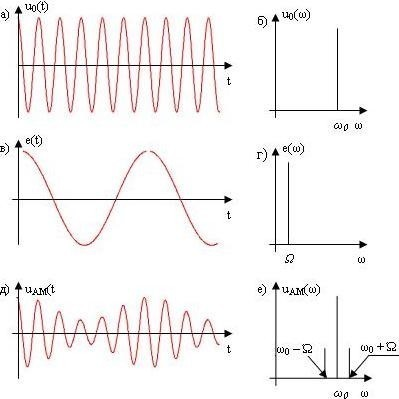
\includegraphics[scale=0.5]{1_1.jpg}}
\caption{Амплитудная модуляция. Несущее колебание(а) и его спектр(б); модулирующий сигнал(в) и его спектр(г); амплитудно-модулирующее колебание(д) и его спектр(е). }
\label{fig:image}
\end{figure} \\

Основными достоинстави амплитудной модуляции являются:
\begin{itemize}
	\item узкая ширина спектра АМ сигнала;
	\item простота получения модулированных сигналов.
\end{itemize}

Недостатками этой модуляции являются:
\begin{itemize}
	\item низкая помехоустойчивость (т. к. при воздействии помехи на сигнал искажается его форма — огибающая, которая и содержит передаваемое сообщение);
	\item неэффективное использование мощности передатчика (т. к. наибольшая часть энергии модулированного сигнала содержится в составляющей несущего сигнала до 64\%, а на информационные боковые полосы приходится по 18\%).
\end{itemize}

\subsubsection{Фазовая модуляция}
{\bf Фазовая модуляция} — один из видов модуляции, при которой фаза несущего колебания управляется информационным сигналом. Фазомодулированный сигнал $S_{ФМн}(t)$ имеет следующий вид: $$S_{ФМн}(t)=s_c(t)\sin[2\pi f_ct + \varphi(t)]$$ где, $s_c(t)$ - огибающая сигнала; $\varphi(t)$ является модулирующим сигналом; $f_c$ - частота несущего сигнала ; $t$ - время.\\
На рисунке преставлена фазовая модуляция и ее спектр:
\begin{figure}[h]
\center{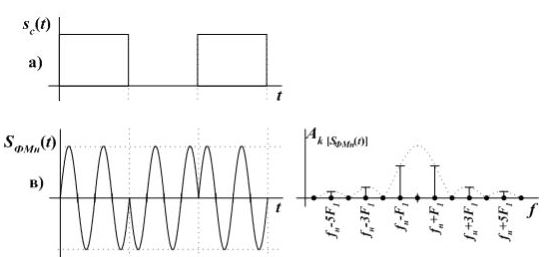
\includegraphics[scale=0.8]{1_3.jpg}}
\caption{Фазовая модуляция и ее спектр.}
\label{fig:image}
\end{figure}
\\
Достоинствами фазовой модуляции являются:
\begin{itemize}
	\item высокая помехоустойчивость;
	\item более эффективное использование мощности передатчика(так как в спектральной характеристике видно почти полное отсутствие несущей).
\end{itemize}
Недостатками фазовой модуляции являются:
\begin{itemize}
	\item большая ширина спектра;
	\item сравнительная трудность получения модулированных сигналов и их детектирование.
\end{itemize}

\subsubsection{Квадратурно-амплитудная модуляция}
{\bf Квадратурная модуляция, квадратурно-амплитудная модуляция} (КАМ, КАМн; англ. {\it Quadrature Amplitude Modulation, QAM}) — разновидность амплитудной модуляции сигнала, которая представляет собой сумму двух несущих колебаний одной частоты, но сдвинутых по фазе относительно друг друга на $90^{\circ}$ ($\frac{\pi}{2}$ радиан, поэтому «квадратурная»), каждое из которых модулировано по амплитуде своим модулирующим сигналом:
$$S(t) = I(t)\cos(2\pi f_0t) + Q(t)\sin(2\pi f_0t),$$
где $I(t)$ и $Q(t)$ - модулирующие сигналы, $f_0$ - несущая частота.\\
\\
{\bf Процесс формирования сигнала.} \\\indent
Предположим, что количество сигналов $q$ равно $2^{m}$, где $m$ показывает число бит, переносимых одним сигналом. Пусть для начала  $m = 2k$, $k$ — натуральное. Тогда $\sqrt{q}=2^{k}$. Тогда сигналу с номером $i$ можно поставить в соответствие два числа  $i_1$ и $i_2$, $i_{1},i_{2} = 0,1,...,{\sqrt q}-1$ по следующему правилу: $i=i_{1}{\sqrt q}+i_{2}$. Пусть
$$
s_{i_1}=A\left(1-\frac{2i_1}{\sqrt{q}-1}\right)\: и\: s_{i_2}=A\left(1-\frac{2i_2}{\sqrt{q}-1}\right)
$$
Тогда величины $s_{{i_{1}}}$ и $s_{{i_{2}}}$ будут равномерно расположены в интервале $[-A,A]$. Минимальное расстояние составит $\Delta ={\frac {2A}{{\sqrt q}-1}}.$

Если $m=2k-1$, то сигнальное множество строится путём прореживания сигнального множества для $ q=2^{{2k}}$. Для этого случая минимальное расстояние $\Delta '={\sqrt 2}\Delta ={\frac {2{\sqrt 2}A}{{\sqrt q}-1}}$ \\
Сигнальное созвездие при $m=4$ представлено на следующем рисунке:
\begin{figure}[h]
\center{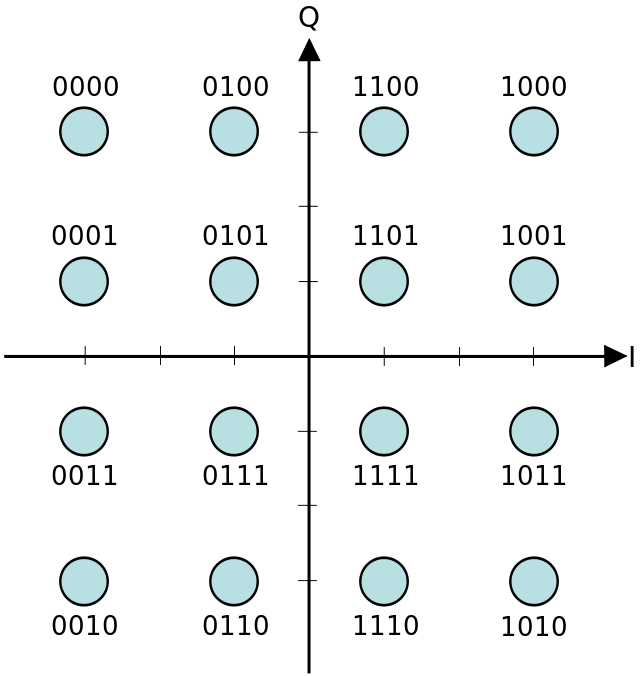
\includegraphics[scale=0.25]{1_2.jpg}}
\caption{Сигнальное созвездие 16-позиционного КАМн-сигнала}
\label{fig:image}
\end{figure}

